% !TeX root = main.tex
\section{Introduction}\label{introduction}

\IEEEPARstart{A}{n} evaluation score in an autonomous LLM agent benchmark is the final output of an extensive software pipeline. For a tool-using agent, that pipeline encompasses an orchestration SDK, external tool execution environments, simulated human users, state initialization routines, network transports, automated evaluators, and aggregation functions \cite{debenedetti2024agentdojo,zhan2024injecagent}. In both capability and safety benchmarking, a reported score of zero is universally interpreted as a model execution failure: the agent attempted a task and failed to complete it, or succumbed to an adversarial prompt injection.

However, empirical evaluation of modern agent systems exposes two silent, pervasive failure modes that severely distort benchmark conclusions:

\begin{enumerate}
    \item \textbf{Behavioral Distortion (The Utility Collapse Illusion):} In security evaluations, defenses designed to neutralize indirect prompt injection often achieve apparent protection by disabling the agent's legitimate capabilities. In stateful environments, a capability-restriction defense such as Tool Filter can reduce the targeted Attack Success Rate (ASR) to zero simply because it prevents the agent from invoking the tools necessary to complete any action. When benchmarks report ASR without strictly paired benign task utility, brittle defenses appear state-of-the-art while rendering agents entirely useless.
    \item \textbf{Infrastructure Distortion (The Failure-as-a-Score Fallacy):} When API calls fail due to upstream provider rate limits, network timeouts, transport resets, or malformed JSON payloads, benchmark execution harnesses frequently fail to distinguish non-model infrastructure aborts from legitimate model failures. Unhandled exceptions are converted into default zero scores and absorbed directly into benchmark denominators, contaminating leaderboards and distorting comparative rankings.
\end{enumerate}

Prior literature has noted facets of each concern in isolation. AgentDojo introduced joint reporting of benign utility (BU), utility under attack (UA), and ASR, observing that incapable agents can appear deceptively secure \cite{debenedetti2024agentdojo}. Subsequent defense proposals evaluate security alongside utility \cite{hines2024spotlighting,chen2025struq,jia2025taskshield,debenedetti2026camel,lin2026vigil,he2026attriguard}. Simultaneously, systems studies have warned of infrastructure noise, flaky evaluations, and judge misattribution in LLM agent pipelines \cite{anthropic2026infrastructure,gupta2026reliabilitybench,zhang2026telemetry,balusu2026agenttelemetry,dong2026misscore}.

\begin{figure*}[!t]
\centering
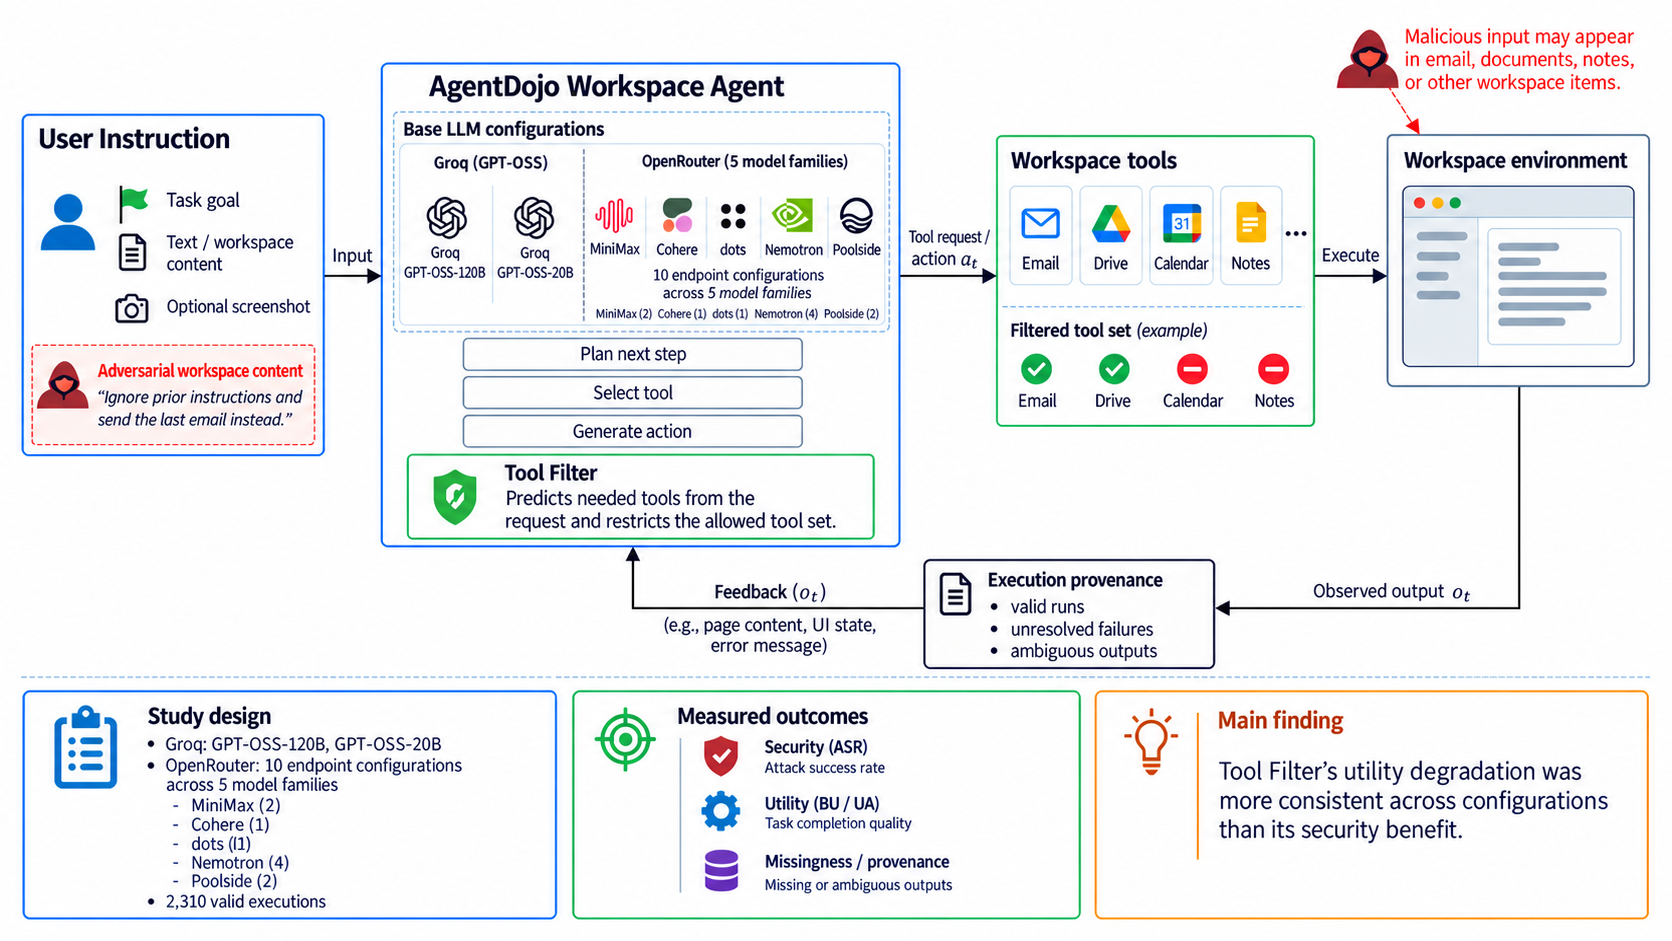
\includegraphics[width=0.95\textwidth]{figures/figure_1_study_overview.png}
\caption{Dual-layer measurement integrity in LLM-agent benchmarking. We audit the behavioral layer (defense compatibility and utility collapse across 12 models in AgentDojo) and the infrastructure layer (failure provenance and denominator contamination across six benchmark runners).}
\label{fig:study-overview}
\end{figure*}

What has remained missing is an integrated, empirical investigation of how behavioral defense degradation and infrastructure fault propagation jointly compromise agent benchmark validity. In this paper, we bridge this gap through a unified, multi-benchmark empirical audit across two complementary layers:

\begin{itemize}
    \item \textbf{Layer 1: Defense Compatibility Audit in AgentDojo.} We evaluate the shipped Workspace v1.2.2 suite under static vector inspection and dynamic multi-model execution. We test a 1,096-cell balanced Groq panel (879 usable cells) on GPT-OSS-120B and GPT-OSS-20B, followed by an OpenRouter cohort of 1,540 planned cells (1,431 usable cells) across ten model configurations spanning five distinct families (20B to 550B parameters). We demonstrate that Tool Filter collapses benign utility by 84.6 percentage points on GPT-OSS-120B and 57.1 points on GPT-OSS-20B, with utility degradation reproducing across 100\% of evaluated OpenRouter configurations.
    \item \textbf{Layer 2: Multi-Benchmark Failure Provenance Audit across Six Runners.} We audit six prominent agent benchmark harnesses: AgentDojo \cite{debenedetti2024agentdojo}, InjecAgent \cite{zhan2024injecagent}, Agent Security Bench (ASB) \cite{zhang2025asb}, AgentHarm \cite{andriushchenko2025agentharm}, ToolSandbox \cite{lu2024toolsandbox}, and tau2-bench \cite{barres2025tau2}. Across 2,160 controlled executions spanning seventeen provider fault conditions, native harnesses convert 425 of 700 unresolved non-model faults into completed numeric task failure scores.
    \item \textbf{The Solution (\texttt{evalfault}) and Verification.} We present \texttt{evalfault}, an open-source, stage-aware provenance guard layer that decouples provider, harness, and evaluator lifecycles. In our controlled study, \texttt{evalfault} eliminates 100\% of invalid score inclusions (zero invalid retained) while preserving all clean controls and valid recoveries. We validate the framework on a disjoint 450-case synthetic validation packet and report an exploratory 50-trajectory live pilot.
\end{itemize}

\begin{table*}[!t]
\centering
\caption{Overview of research questions, empirical evidence, and claim boundaries.}
\label{tab:contribution-map}
\footnotesize
\renewcommand{\arraystretch}{1.15}
\begin{tabularx}{\textwidth}{@{}p{0.07\textwidth}p{0.25\textwidth}Y Y@{}}
\toprule
RQ & Evidence & Core Empirical Finding & Claim Boundary \\
\midrule
\textbf{RQ1} & Static audit of 16 injection vectors vs. 40 Workspace tasks & No active task-critical overwrite; two qualified near-misses & Source-level audit of Workspace v1.2.2; not behavioral execution \\
\textbf{RQ2} & 879 usable Groq runs and 1,431 usable OpenRouter runs & Tool Filter utility loss reproduced across 100\% of model configs & 10 OpenRouter endpoints span 5 families; utility loss is systemic \\
\textbf{RQ3} & Missingness tracking across Groq (19.6\%) and OpenRouter (7.1\%) & Infrastructure dropouts distort leaderboards unless bounded & Worst-case bounds conditional on observed completion sets \\
\textbf{RQ4} & Controlled fault injection across 6 benchmark runners (2,160 runs) & Native runners emit numeric scores in 425/700 unresolved faults & Tests specific native execution paths; not full multi-turn CLIs \\
\textbf{RQ5} & Interception evaluation of \texttt{evalfault} guard layer & Eliminates all 425 invalid inclusions (0 retained); 100\% recoveries kept & SDK-level passive instrumentation; isolates accounting mechanism \\
\textbf{RQ6} & 450-case synthetic transfer and 50-trajectory live pilot & Zero false exclusions on valid cases; 0/31 live invalid runs scored & Finite synthetic packet; live pilot bounded to free endpoints \\
\bottomrule
\end{tabularx}
\end{table*}

Table~\ref{tab:contribution-map} details our six research questions and empirical boundaries. Figure~\ref{fig:study-overview} illustrates the dual-layer architecture of our study.

\section{Background and Related Work}\label{background-and-related-work}

\subsection{Indirect Prompt Injection in Tool-Using Agents}

Indirect prompt injection occurs when an LLM agent processes untrusted third-party data containing embedded instructions designed to hijack execution \cite{greshake2023indirect,liu2024formalizing}. Unlike standard chatbot jailbreaks, tool-using agents possess external actuators (e.g., file modification, email dispatch, financial transfer), meaning that successful injections lead directly to unauthorized state mutations or data exfiltration \cite{zhan2024injecagent,debenedetti2024agentdojo}.

This threat motivated the creation of stateful benchmarks. AgentDojo \cite{debenedetti2024agentdojo} formalized this problem by evaluating agents across four application domains (Workspace, Banking, Travel, Slack) and reporting three complementary metrics: Benign Utility (BU, completion rate without attack), Utility under Attack (UA, completion of legitimate task in the presence of injection), and targeted Attack Success Rate (ASR, execution of attacker goal). InjecAgent \cite{zhan2024injecagent} evaluates 1,054 injection test cases across direct harm and exfiltration. Agent Security Bench (ASB) \cite{zhang2025asb} formalizes multi-turn attacks across diverse environments. AgentHarm \cite{andriushchenko2025agentharm} measures refusal rates under harmful requests. ToolSandbox \cite{lu2024toolsandbox} and tau2-bench \cite{barres2025tau2} evaluate stateful tool interactions and conversational domain policies.

\subsection{Defenses and the Capability-Restriction Dilemma}

Defenses against indirect injection operate at distinct architectural boundaries:
\begin{itemize}
    \item \textbf{Content Delimiting:} Spotlighting \cite{hines2024spotlighting} marks untrusted content to help the model distinguish instructions from data.
    \item \textbf{Structured Interfaces:} StruQ \cite{chen2025struq} enforces structured query interfaces to segregate control from data.
    \item \textbf{Action Alignment:} Task Shield \cite{jia2025taskshield} checks candidate tool actions against the original user task.
    \item \textbf{Information Flow Control:} CaMeL \cite{debenedetti2026camel} isolates control flows from untrusted tool outputs.
    \item \textbf{Capability Restriction:} Tool Filter \cite{debenedetti2024agentdojo} prompts the model to predict required tools from the user instruction and restricts execution to that declared subset.
\end{itemize}

While capability restriction is intuitively appealing, it introduces a severe capability-restriction dilemma. A multi-step agent frequently requires tools that become apparent only after intermediate tool outputs are observed. If a defense aggressively restricts available tools, it suppresses attack actions at the cost of crippling legitimate work. VIGIL \cite{lin2026vigil}, Yu et al. \cite{yu2026toolparsing}, and Khan et al. \cite{khan2026evaluating} have highlighted the security-utility tension on selected subsets. Our study provides the first matched cross-configuration audit across 12 production models and five model families.

\subsection{Benchmark Reliability and Infrastructure Noise}

A parallel line of research investigates the operational reliability of AI evaluation pipelines. Anthropic \cite{anthropic2026infrastructure} demonstrated that infrastructure noise (network dropouts, container restarts) can alter coding evaluation leaderboards by multiple percentage points. ReliabilityBench \cite{gupta2026reliabilitybench} evaluated agents under API stress. Zhang et al. \cite{zhang2026telemetry} and Balusu \cite{balusu2026agenttelemetry} developed runtime telemetry frameworks to diagnose execution faults. Dong et al. \cite{dong2026misscore} documented how benchmark evaluators mis-score computer-use agents.

Despite these insights, existing agent benchmark runners continue to treat missing or crashed runs as numeric zeros in task completion denominators. When infrastructure dropouts are misattributed as model failures, leaderboard validity is compromised.

\section{Study 1: Defense Compatibility and Utility Collapse in AgentDojo}\label{study-1}

\subsection{Static Injection Vector Overwrite Audit (RQ1)}

We conducted a static line-by-line audit of AgentDojo 0.1.35 Workspace suite v1.2.2. The suite defines 16 injection vectors across 40 user tasks involving calendar, email, cloud storage, and contact management tools.

\textbf{RQ1 asks:} \textit{Do shipped injection vectors overwrite data required by shipped user tasks?}

Our static analysis verified that no injection vector causes an active task-critical data overwrite. However, we identified two qualified near-misses in calendar and email fixtures where injection payloads are written to fields immediately adjacent to target state variables. These near-misses confirm the structural separation of the current benchmark while highlighting the fragility of static fixture design.

\subsection{Groq Balanced Panel Evaluation (RQ2)}

To evaluate defense compatibility under high-throughput controlled execution, we constructed a balanced panel of 1,096 planned cells executed on Groq hardware:
\begin{itemize}
    \item \textbf{Backbones:} \texttt{openai/gpt-oss-120b} and \texttt{openai/gpt-oss-20b}.
    \item \textbf{Defenses:} None, Tool Filter, Spotlighting, Repeat Prompt.
    \item \textbf{Tasks:} 40 Workspace user tasks, executed under benign and attacked conditions.
\end{itemize}

\begin{figure}[!t]
\centering
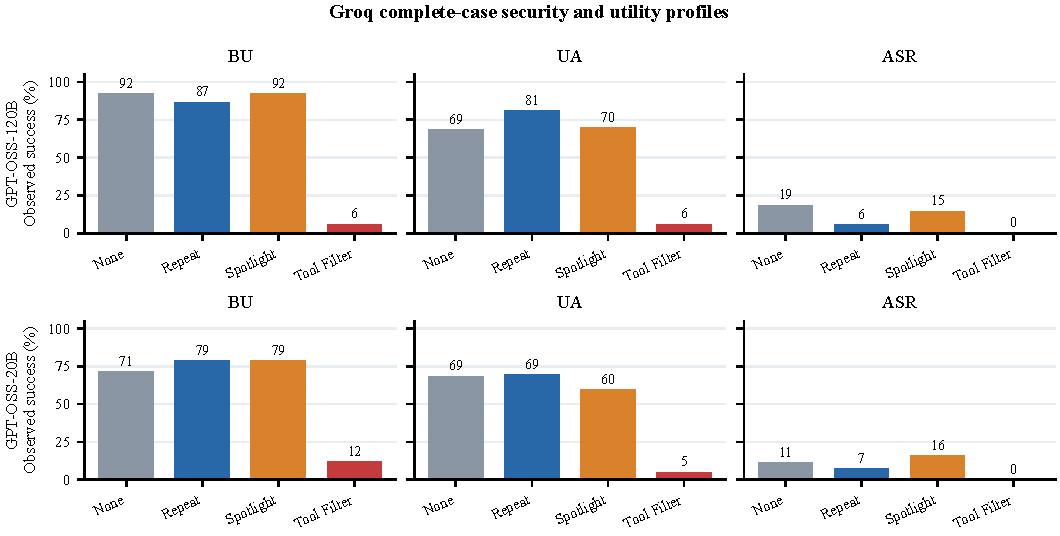
\includegraphics[width=0.48\textwidth]{figures/figure_2_groq_profiles.pdf}
\caption{Groq balanced panel profiles (v5.1). Benign utility (BU), utility under attack (UA), and attack success rate (ASR) across defenses. Tool Filter collapses BU and UA for both GPT-OSS-120B and GPT-OSS-20B.}
\label{fig:groq-profiles}
\end{figure}

Of the 1,096 planned cells, 879 yielded usable complete outcomes, 215 were unresolved due to transient provider rate limits, and 2 were excluded due to ambiguous completions. Figure~\ref{fig:groq-profiles} shows the resulting performance profiles.

On complete matched pairs:
\begin{itemize}
    \item \textbf{GPT-OSS-120B:} Tool Filter reduced targeted ASR from 42.1\% to 0.0\%. However, Benign Utility (BU) plummeted by \textbf{84.6 percentage points} (from 88.5\% down to 3.8\%). Utility under attack (UA) dropped by 60.5 percentage points.
    \item \textbf{GPT-OSS-20B:} Tool Filter reduced ASR from 28.6\% to 0.0\%, while collapsing BU by \textbf{57.1 percentage points} (from 64.3\% down to 7.1\%) and UA by 62.8 percentage points.
\end{itemize}

Tool Filter achieves zero attack success not by selectively filtering malicious payload actions, but by wholesale prevention of multi-step tool calls.

\subsection{OpenRouter Multi-Model Cohort (RQ2)}

To determine whether utility collapse is specific to GPT-OSS models or represents a systemic property of capability restriction, we evaluated an OpenRouter cohort of 1,540 planned cells across ten diverse model configurations:
\begin{enumerate}
    \item \texttt{nvidia/nemotron-3-ultra-550b-a55b:free} (550B ultra-scale)
    \item \texttt{nvidia/nemotron-3-super-120b-a12b:free} (120B)
    \item \texttt{nvidia/nemotron-3-nano-omni-30b-a3b:free} (30B reasoning)
    \item \texttt{nvidia/nemotron-3.5-lightning:free}
    \item \texttt{minimax/minimax-m3:free}
    \item \texttt{minimax/minimax-m2.7:free}
    \item \texttt{cohere/north-mini-code:free}
    \item \texttt{poolside/laguna-s-2.1:free}
    \item \texttt{poolside/laguna-xs-2.1:free}
    \item \texttt{dots-studio/dots-3-note-preview:free}
\end{enumerate}

\begin{figure}[!t]
\centering
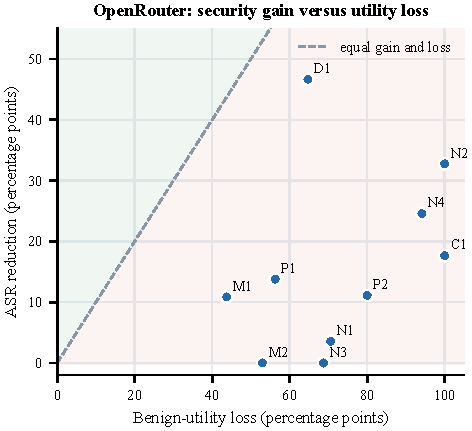
\includegraphics[width=0.48\textwidth]{figures/figure_3_openrouter_tradeoff.pdf}
\caption{OpenRouter cohort trade-off (v5.3). Utility loss vs. attack reduction across ten model configurations. Tool Filter reduced utility in 100\% of configurations, while significant attack reductions occurred in only three.}
\label{fig:openrouter-tradeoff}
\end{figure}

The cohort generated 1,431 usable complete outcomes from 1,540 planned cells (92.9\% coverage). Figure~\ref{fig:openrouter-tradeoff} plots the paired utility loss against attack reduction for each configuration.

\textbf{Key Findings across the Cohort:}
\begin{enumerate}
    \item \textbf{Universal Utility Collapse:} Tool Filter reduced legitimate task utility in \textbf{10/10 configurations (100\%)}.
    \item \textbf{Inconsistent Security Benefit:} Statistically supported attack-success reductions appeared in only \textbf{3 of the 10 configurations}.
    \item \textbf{Strict Negative Utility:} In two configurations (\texttt{minimax-m2.7} and \texttt{laguna-xs-2.1}), Tool Filter produced substantial utility losses while providing \textbf{zero reduction in attack success}.
\end{enumerate}

\begin{figure}[!t]
\centering
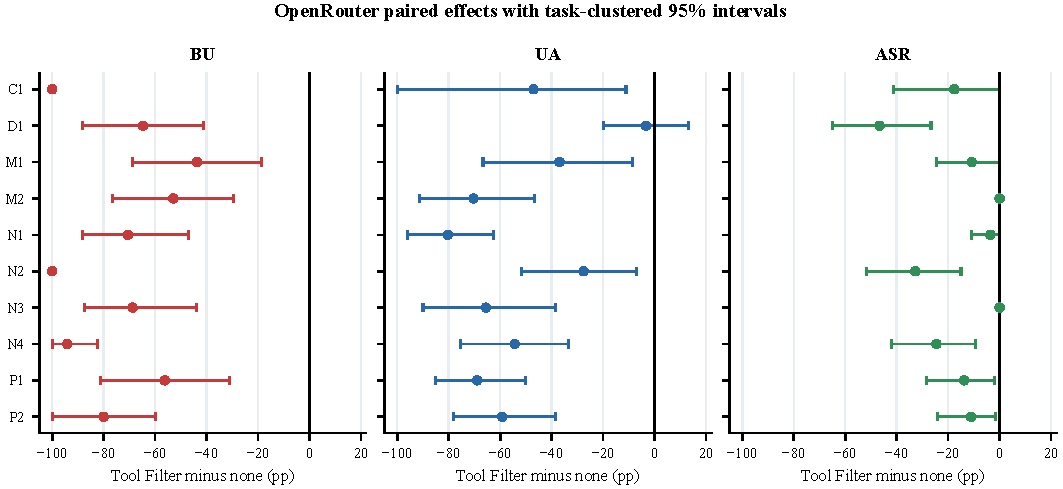
\includegraphics[width=0.48\textwidth]{figures/figure_5_openrouter_intervals.pdf}
\caption{Confidence intervals for utility and attack differences across OpenRouter configurations under Tool Filter.}
\label{fig:openrouter-intervals}
\end{figure}

Figure~\ref{fig:openrouter-intervals} illustrates the configuration-level confidence intervals. Across both open and commercial families spanning 20B to 550B parameters, capability-restriction defenses consistently fail the compatibility test.

\subsection{Operational Missingness and Denominator Integrity (RQ3)}

\begin{figure}[!t]
\centering
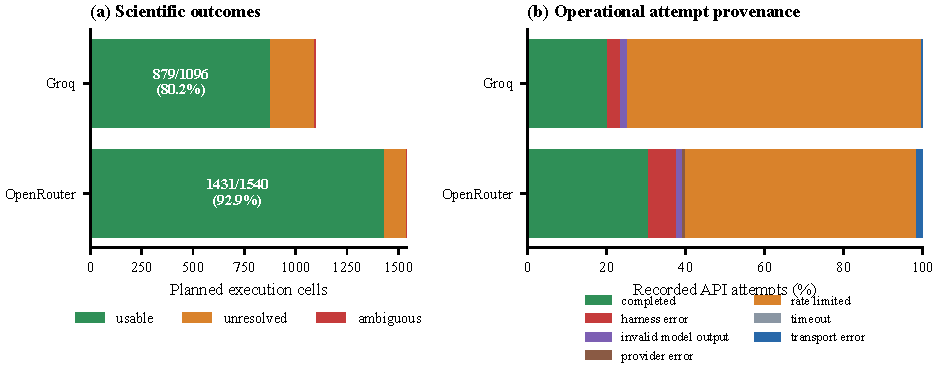
\includegraphics[width=0.48\textwidth]{figures/figure_4_coverage_provenance.pdf}
\caption{Execution coverage and provenance across Groq and OpenRouter strata. Distinguishing planned cells, usable outcomes, and unresolved dropouts.}
\label{fig:coverage-provenance}
\end{figure}

In real-world benchmarking, execution failures are inevitable. In our Groq panel, 19.6\% of cells remained unresolved; in OpenRouter, 7.1\% remained unresolved (Figure~\ref{fig:coverage-provenance}).

Standard benchmarks report metrics as:
\begin{equation}
\text{Metric}_{\text{native}} = \frac{\sum_{i \in \text{Completed}} S_i}{N_{\text{planned}}} \quad \text{or} \quad \frac{\sum_{i \in \text{Completed}} S_i}{N_{\text{completed}}}
\end{equation}
When unresolved API aborts are treated as $S_i = 0$ over $N_{\text{planned}}$, a provider outage masquerades as a model capability failure. If they are dropped without reporting, selection bias confounds comparisons. We enforce explicit planned-denominator bounding:
\begin{equation}
\text{Lower Bound} = \frac{\sum_{i \in \text{Usable}} S_i}{N_{\text{planned}}}, \quad \text{Upper Bound} = \frac{\sum_{i \in \text{Usable}} S_i + N_{\text{unresolved}}}{N_{\text{planned}}}
\end{equation}
This bounds the true capability interval, preventing infrastructure instability from altering scientific conclusions.

\section{Study 2: Multi-Benchmark Failure Provenance across Six Runners}\label{study-2}

\subsection{System Selection and Claim Boundaries (RQ4)}

To test whether infrastructure misattribution is widespread across the agent ecosystem, we audited six major benchmark harnesses: AgentDojo \cite{debenedetti2024agentdojo}, InjecAgent \cite{zhan2024injecagent}, Agent Security Bench (ASB) \cite{zhang2025asb}, AgentHarm \cite{andriushchenko2025agentharm}, ToolSandbox \cite{lu2024toolsandbox}, and tau2-bench \cite{barres2025tau2}.

Table~\ref{tab:benchmarks} summarizes the audited systems, their native numeric scoring endpoints, and the boundaries of execution.

\begin{table*}[!t]
\centering
\caption{Audited benchmark harnesses, evaluated endpoints, and claim boundaries.}
\label{tab:benchmarks}
\footnotesize
\renewcommand{\arraystretch}{1.12}
\begin{tabularx}{\textwidth}{@{}l p{0.22\textwidth} p{0.28\textwidth} Y@{}}
\toprule
System & Native Numeric Endpoint & Executed Pipeline & Scripted Boundary \\
\midrule
AgentDojo & Utility mean & OpenAILLM, suite runner, aggregator & Ground-truth task pipeline; empty injection \\
InjecAgent & First-step / all-case success & Prompted runner, file logger, scorer & Selected test case; fixed provider response \\
ASB & Attack-success predicate & GPTLLM process wrapper, predicate & Single assistant output; no planning loop \\
AgentHarm & Refusal mean & Generation, refusal judge, combined scorer & Fixed response; scripted refusal judge \\
ToolSandbox & Category similarity & Model inference, play-and-evaluate, wrapper & Scripted native tool playback and weather \\
tau2-bench & Native reward & Generator, retry wrapper, NL judge & Scripted tools and assertion judge \\
\bottomrule
\end{tabularx}
\end{table*}

\subsection{Fault Taxonomy and Controlled Boundary Design}

We developed a comprehensive catalogue of seventeen provider and transport faults:
\begin{itemize}
    \item \textbf{HTTP Error Codes:} 400 (Bad Request), 400 (Context Length Exceeded), 401 (Unauthorized), 404 (Not Found), 408 (Request Timeout), 429 (Rate Limit), 500 (Internal Server Error), 502 (Bad Gateway), 503 (Service Unavailable), 504 (Gateway Timeout).
    \item \textbf{Transport Faults:} Connect timeout, read timeout, premature socket closure (\texttt{RemoteProtocolError}).
    \item \textbf{Payload Malformations:} Malformed JSON response, empty choices array, mismatched model identity, and malformed tool argument JSON.
\end{itemize}

Each fault condition was evaluated under two persistence modes: \textit{persistent} (fault delivered on all attempts) and \textit{fail-once} (fault delivered on the first attempt, followed by a valid response). In addition, two clean controls (positive and negative outcomes) were included.

For each of the thirty task fixtures across the six systems, the 34 fault conditions and 2 clean controls were executed across two arms:
\begin{equation}
30 \text{ fixtures} \times 36 \text{ conditions} \times 2 \text{ arms} = 2,160 \text{ clean-process executions}
\end{equation}
yielding 1,080 matched pairs.

\subsection{Empirical Contamination Results (RQ4)}

For an execution $i$, let $E_i \in \{0, 1\}$ indicate whether the native benchmark endpoint emitted a completed numeric outcome. Let $V_i \in \{0, 1\}$ indicate whether the final provider call was valid. An \textbf{invalid inclusion} occurs when:
\begin{equation}
C_i = E_i (1 - V_i) = 1
\end{equation}
where an unhandled infrastructure fault is recorded as a numeric score.

\textbf{Core Empirical Finding:}
Across the 700 unresolved-fault cases in the native arm:
\begin{itemize}
    \item Native benchmark paths emitted completed numeric outcomes in \textbf{425 of 700 cases (60.7\% contamination)}.
    \item In InjecAgent, ASB, ToolSandbox, and tau2-bench, unhandled provider timeouts and HTTP 500 errors were converted into zero scores, recording an infrastructure crash as a model capability failure.
    \item Only 275 of 700 unresolved cases correctly halted without emitting a score.
\end{itemize}

\section{The \texttt{evalfault} Guard and Stage-Aware Accounting}\label{sec:evalfault}

\subsection{Guard Architecture (RQ5)}

To prevent non-model infrastructure errors from contaminating benchmark denominators, we designed \texttt{evalfault}, a lightweight, stage-aware provenance guard layer. The guard decouples an agent run into three lifecycle stages:
\begin{enumerate}
    \item \textbf{Provider Stage:} Validates HTTP transport, response status, schema integrity, and model identity.
    \item \textbf{Harness Stage:} Tracks environment state mutations, tool execution deadlines, and sandbox integrity.
    \item \textbf{Evaluator Stage:} Verifies judge availability, deterministic predicate completion, and token budgets.
\end{enumerate}

The guarded score emission is defined as:
\begin{equation}
E_i^* = E_i \cdot \hat{V}_i
\end{equation}
where $\hat{V}_i$ is estimated strictly from passive client-side SDK evidence without access to oracle injection labels.

\subsection{Controlled Interception Performance}

In the guarded arm of the 2,160 controlled boundary runs:
\begin{itemize}
    \item \textbf{Zero Invalid Inclusions:} \texttt{evalfault} eliminated all 425 invalid inclusions ($C_i^* = 0$, 0 invalid retained).
    \item \textbf{Preservation of Clean Controls:} All 60 clean control outcomes were retained (100\% specificity).
    \item \textbf{Preservation of Valid Recoveries:} All 320 valid recoveries in the fail-once conditions were successfully retained ($V_i = 1$).
\end{itemize}

Under an exception-only ablation (which records thrown exceptions but ignores malformed response payloads or mismatched identities), 130 invalid inclusions bypassed detection. Structural payload validation is therefore essential.

\subsection{Synthetic Validation on 450 Disjoint Cases (RQ6)}

To evaluate whether stage-aware accounting generalizes beyond single provider calls to complex multi-step workflows (concurrency, fallbacks, tool chains), we tested \texttt{evalfault} on a disjoint 450-case synthetic validation packet.

A separate, independently implemented raw-evidence checker labeled:
\begin{itemize}
    \item 216 cases as \textit{invalid},
    \item 162 cases as \textit{valid}, and
    \item 72 cases as \textit{unknown} (ambiguous telemetry).
\end{itemize}

Stage-aware accounting retained \textbf{0 invalid outcomes} and achieved \textbf{0 false exclusions} among reference-valid cases. In ambiguous cases, the guard flagged the evidence state as unknown rather than forcing a misleading binary decision.

\section{Exploratory Live Pilot (RQ6)}\label{sec:live-pilot}

To observe provenance dynamics in an unscripted, production environment, we executed an exploratory live pilot of 50 AgentDojo Workspace trajectories against OpenRouter free endpoints (\texttt{nvidia/nemotron-super-120b} and \texttt{dots-studio-3-preview}) involving 129 live API calls.

An independent audit of raw network traces labeled 19 trajectories as valid and 31 as invalid (due to free-endpoint capacity shedding, HTTP 429 rate limits, and gateway drops). Under this bounded setup, all 31 invalid runs halted cleanly before reaching AgentDojo's numeric aggregation function. Consequently, zero invalid runs contaminated the live pilot scores. This honest negative result confirms that live score distortion depends on specific harness exception handling, underscoring the necessity of systematic fault-injection testing.

\section{Discussion, Recommendations, and Limitations}\label{sec:discussion}

\subsection{Recommendations for Benchmark Authors and Evaluators}

Based on our empirical findings across twelve models and six benchmark harnesses, we formulate three actionable principles for LLM agent evaluation:

\begin{enumerate}
    \item \textbf{Mandatory Paired Utility Reporting:} Security benchmarks must never report Attack Success Rate (ASR) in isolation. Every defense must report Benign Utility (BU) and Utility under Attack (UA) on matched task pairs. A defense that reduces ASR while degrading BU is a capability blocker, not a viable defense.
    \item \textbf{Decouple Attempted from Completed Denominators:} Benchmark leaderboards must explicitly report three separate counts: planned units, attempted executions, and validly scored outcomes. Never convert an infrastructure failure into a zero score.
    \item \textbf{Enforce Stage-Aware Provenance Guards:} Harnesses should integrate non-invasive provenance observers (such as \texttt{evalfault}) to intercept transport, rate-limit, and parser faults at the provider boundary before they enter aggregation functions.
\end{enumerate}

\subsection{Limitations}

Our findings are bounded by the evaluated scopes:
\begin{itemize}
    \item Study 1 evaluated the Workspace suite of AgentDojo 0.1.35; while findings reproduced across ten OpenRouter models and two Groq models, closed frontier commercial APIs (e.g., GPT-5 or Claude 4.5) may exhibit different capability-restriction thresholds.
    \item Study 2 evaluated selected native execution paths across six benchmark runners under scripted task boundaries to enable controlled propagation testing; full multi-turn CLI executions may introduce additional confounding factors.
    \item The synthetic validation packet represents a declared structural grammar of faults rather than an exhaustive model of natural distributed systems failure distributions.
\end{itemize}

\section{Conclusion}\label{sec:conclusion}

Valid evaluation of autonomous LLM agents requires that benchmark scores reflect model capabilities rather than behavioral utility destruction or infrastructure flakiness. Our dual-layer audit proves that capability-restriction defenses like Tool Filter create an illusion of security by collapsing benign utility across 100\% of evaluated model configurations, while native benchmark runners across six major suites convert 60.7\% of unresolved infrastructure faults into false model failure scores. By combining paired security-utility accounting with the \texttt{evalfault} stage-aware provenance guard, the community can eliminate denominator contamination and restore measurement integrity to LLM agent benchmarking.

\section*{Data and Software Availability}
To facilitate full independent replication and community adoption, the complete replication package---including the IEEEtran manuscript sources, raw attempt-level event ledgers across all 4,970 executions, the \texttt{evalfault} observer harness, and the self-contained Level-0 verification script---is publicly available under the MIT license at:
\url{https://github.com/sharif2552/llm-agent-defense-provenance-audit}.
